\chapter{پیاده سازی و نتایج}

\section{پیاده سازی پلتفرم}
\subsection{سیستم مدیریت}

در پلتفرم‌های بزرگ، نیاز به سیستمی برای مدیریت پلتفرم به وضوح احساس می‌شود. این سیستم باید قابلیت هماهنگی و یکپارچگی بین اجزای مختلف را داشته باشد تا اطمینان حاصل شود که همه بخش‌ها به درستی و بدون مشکل عمل می‌کنند. ویژگی‌های حیاتی این سیستم شامل استفاده از ابزارهای خودکارسازی و نظارت پیشرفته، مدیریت بهینه منابع سخت افزاری، پیاده‌سازی فرآیندهای مستمر بهبود و به‌روزرسانی، مدیریت دسترسی‌ها و امنیت و مستندسازی فرآیندها و تغییرات است. سیستم مدیریت شامل تمامی ابزارهای مدیریتی مانند مدیریت مخازن مولفه‌ها، کد و خط لوله \lr{CI/CD}، مانیتورینگ کل سیستم و جمع آوری لاگ است. علاوه بر این، استراتژی استقرار پروژه، اعمال مهاجرت‌ها\footnote{\lr{Migrations}}، پیکربندی پروژه‌ها، مدیریت سرورهای \lr{DNS} و \lr{NTP}\footnote{\lr{Network Time Protocol}} و استفاده از ابزارهایی مانند \lr{Foreman} برای نصب سیستم‌عامل به صورت \lr{PXE} نیز توسط همین سیستم مدیریت می‌شود.

به منظور پیاده سازی این سیستم، ما دو ماشین مجزا برای مدیریت پلتفرم به منظور ایجاد قابلیت تحمل خطا\footnote{\lr{Fault Tolerance}} و دسترسی پذیری بالا\footnote{\lr{High Availability}}  قرار می‌دهیم. از آنجایی که فرآیند و پروسه سنگینی روی این ماشین ها انجام نمی شود مشخصات کمتری می تواند به نسبت ماشین های پروژه داشته باشد. مشخصات سخت افزاری هرکدام از این ماشین ها در جدول
~\ref{tb: management conf}
قرار دارد.  این ماشین ها به صورت ماشین مجازی با استفاده از \lr{OpenStack} ساخته می شود. ماشین‌های مدیریت باید برای نصب و راه‌اندازی ابزارهای مدیریت پلتفرم پیکربندی شوند و این کار با استفاده از ابزار \lr{Ansible} انجام می گیرد. به این منظور \lr{Role} های مشخصی برای هر بخش نوشته شده است تا بتوان بدون هیچ کار دستی و به صورت کاملا خودکار سیستم ها را پیکربندی کرد. این \lr{Role} های انسیبلی با استفاده از قاعده نسخه گذاری \lr{Semantic} نسخه گذاری شده و در مخزن \lr{raw} موجود در \lr{Nexus} که یک ابزار مدیریت مخازن مولفه می باشد نگه داری خواهند شد. در نهایت برای پیکربندی سیستم، \lr{Role} موردنظر با نسخه مشخص از \lr{Nexus} گرفته شده و بااستفاده از \lr{Ansible} ماشین ها پیکربندی می شوند. از آنجایی که این پیکربندی در محیط های مختلف مانند توسعه و عملیات می تواند متفاوت باشد، ما با استفاده از قابلیت \lr{Overriding} در این ابزار مقادیر پیش فرض را برای هر محیط تغییر خواهیم داد. به همین منظور اسکریپتی طراحی شده که در لینک 
گیت هاب\footnote{\url{https://github.com/abolfazlyarian/mlops.git}} قابل مشاهده است.

\begin{table}
	\centering
	\caption{مشخصات سخت افزاری ماشین های مدیریت}
	\label{tb: management conf}
	\begin{tabular}{|c|c|c|c|}
		\hline
		\lr{OS} & \lr{Storage} &  \lr{RAM} & \lr{CPU} \\ \hline
		\lr{Ubuntu 18.04} & \lr{512 GB} & \lr{8 GB} & \lr{4 Core} \\ \hline
	\end{tabular}
\end{table}

پروسه پیکربندی و نصب ابزار در ماشین های مدیریت به صورت زیر انجام می گردد:
\begin{enumerate}
	\item 
	پیکربندی ماشین ها:
این قسمت شامل نصب و پیکربندی ابزارهایی نظیر
\lr{BIND}
برای سرور \lr{DNS}،
\lr{APT}
برای مدیریت ابزار در سیستم عامل \lr{Ubuntu}،
\lr{pip}
برای مدیریت کتابخانه ها پایتون،
\lr{chrony}
برای سرور \lr{NTP}
،\lr{LDAP} 
برای مدیریت کاربران و … می باشد.
	\item
نصب و پیکربندی \lr{Docker}: از آنجایی که مدیریت ابزارها به صورت کانتینر مناسب تر است، برای انجام مراحل بعدی نیاز به نصب \lr{Docker} می باشد. پس از نصب به منظور ذخیره سازی تمام مولفه ها مورد استفاده به مخزن ساخته شده در \lr{Nexus} مدیریت متصل خواهد شد.
	\item 
 \lr{Nexus}: از این ابزار به منظور مدیریت مخازن مولفه ها استفاده شده است. مخازن مورد استفاده ما \lr{APT}، 
	\lr{pip}،
	\lr{Docker}
	و \lr{raw} می باشد (شکل 
	~\ref{fig: nexus repo}).

	\item 
 \lr{Jenkins}: از این ابزار به منظور اجرا و مدیریت خط لوله های \lr{CI/CD} پروژها و هم چنین پیکربندی آن ها توسط مدیران سیستم استفاده می شود (شکل 
	~\ref{fig: jenkins}).
	
	\item 
 \lr{GitLab}: به منظور مدیریت کد در پروژه ها و هم چنین مدیریت \lr{Role}های انسیبلی برای پیکربندی پروژها استفاده می شود (شکل 
	~\ref{fig: gitlab}).
	
\begin{figure}[!t]
	\centering
	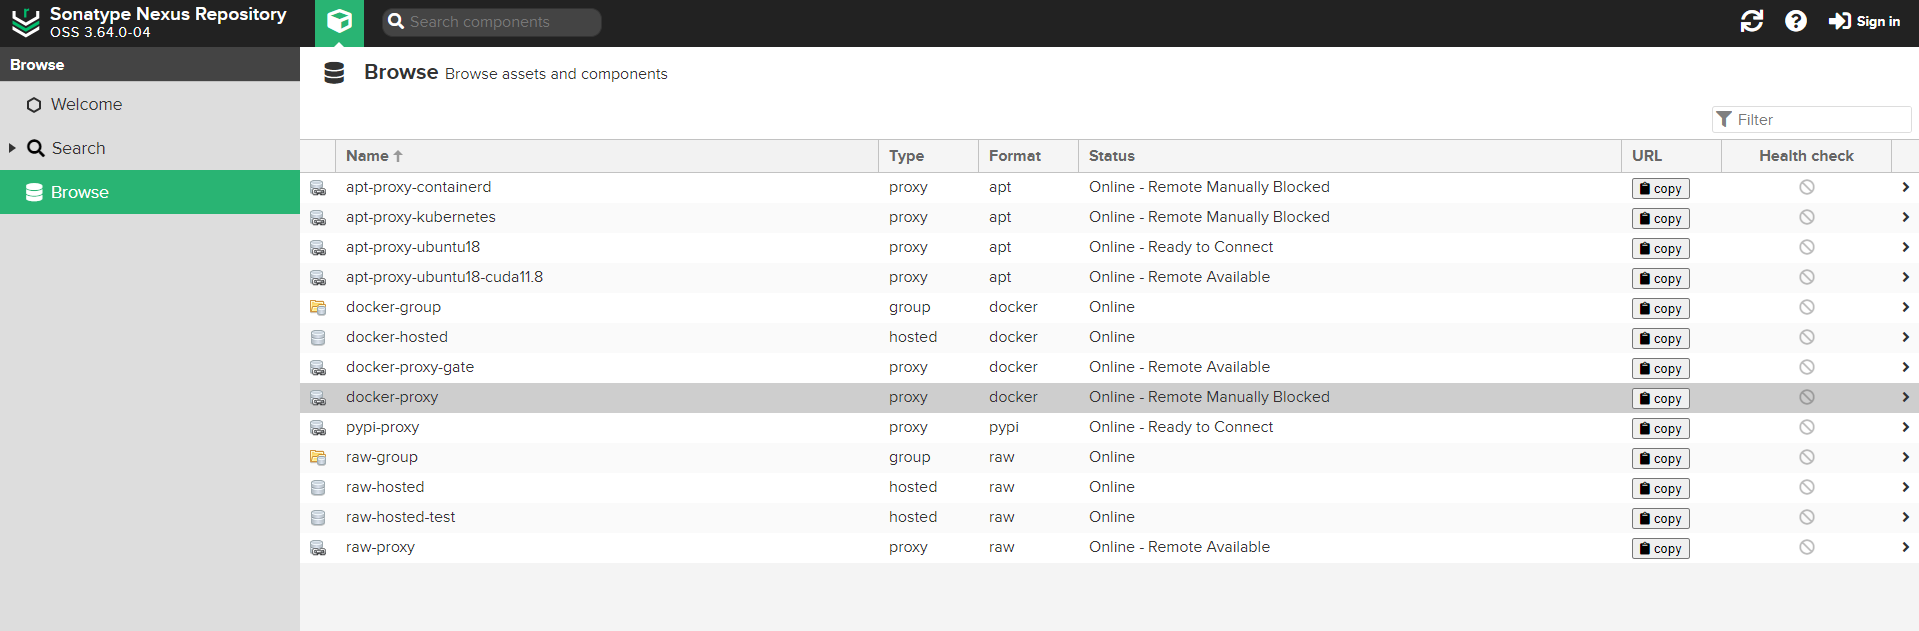
\includegraphics[scale=0.3]{nexus-repo.png}
	\caption{مخازن مولفه در \lr{Nexus}}
	\label{fig: nexus repo}
\end{figure}
\begin{figure}[!t]
	\centering
	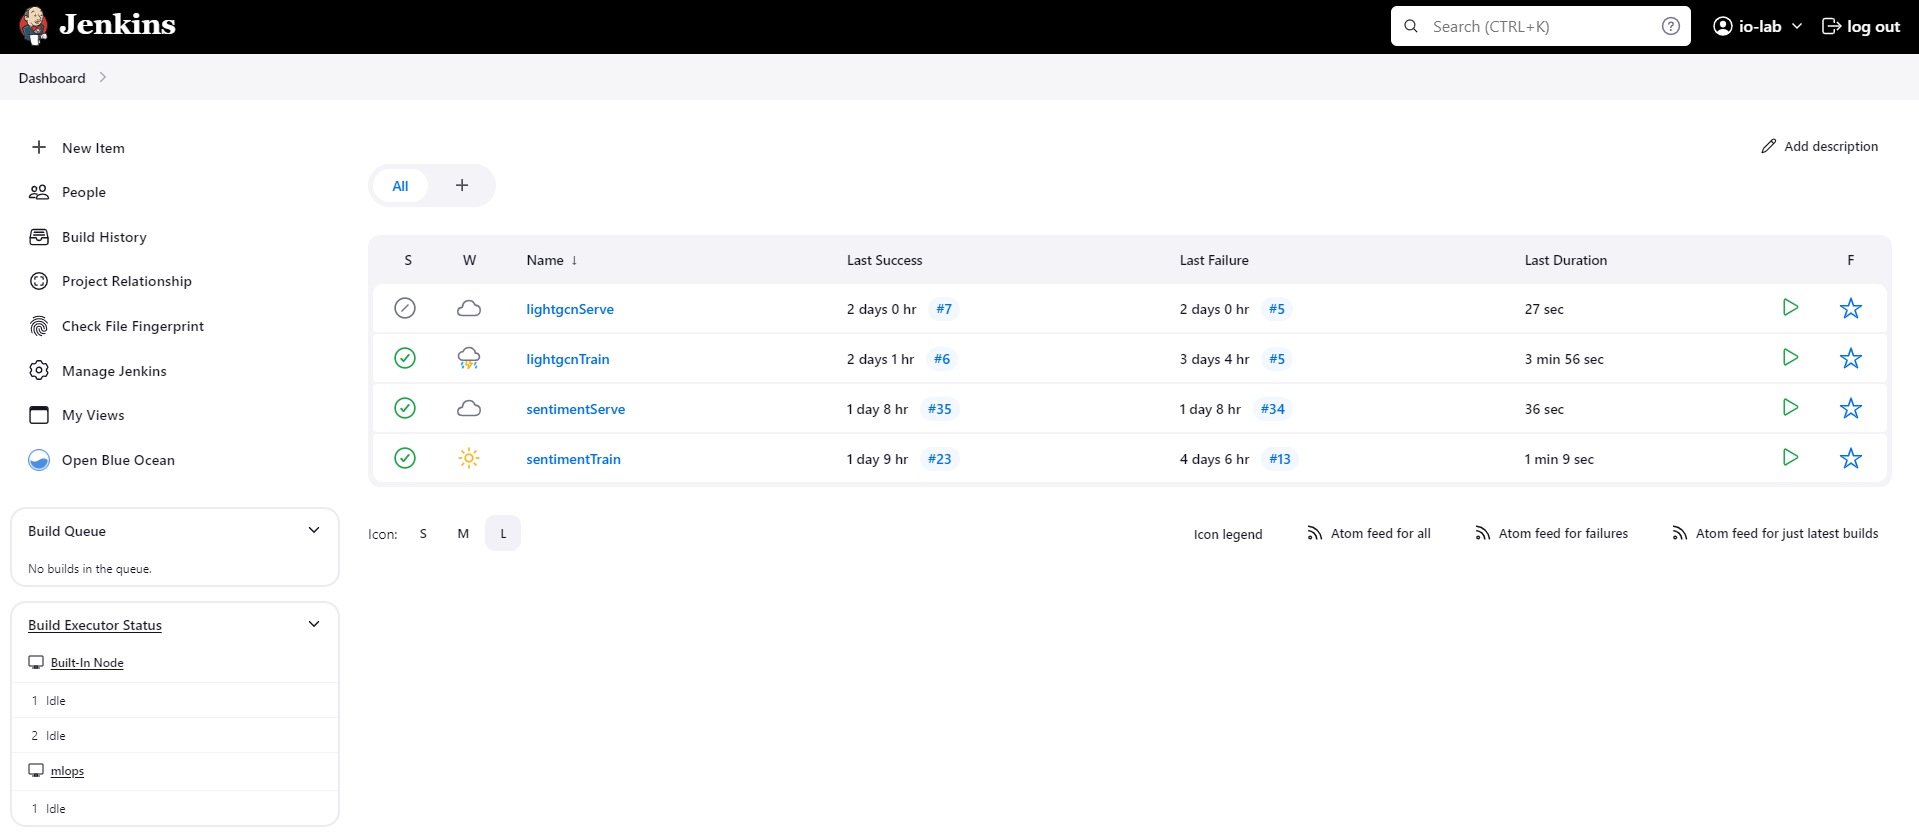
\includegraphics[scale=0.3]{jenkins1.png}
	\caption{خط لوله ها \lr{CI/CD} در \lr{Jenkins}}
	\label{fig: jenkins}
\end{figure}
\begin{figure}[!t]
	\centering
	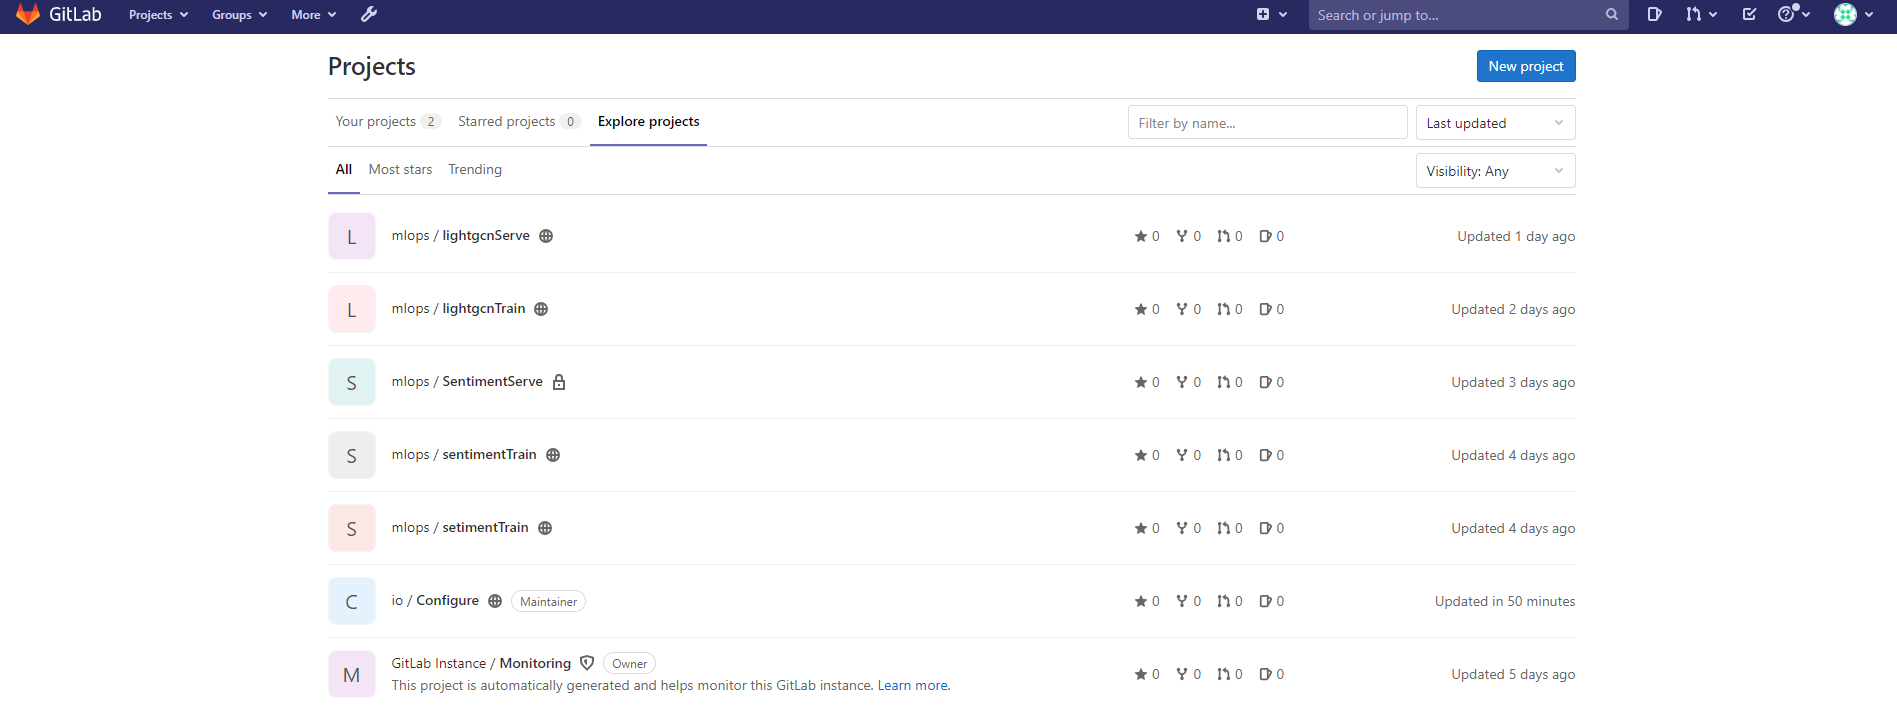
\includegraphics[scale=0.3]{gitlab.png}
	\caption{مخازن کد در \lr{Gitlab}}
	\label{fig: gitlab}
\end{figure}
\end{enumerate}
\clearpage
\subsection{خوشه کوبرنتیز}
در طراحی یک پلتفرم \lr{MLOps} جامع و کارآمد که تمامی ابزارهای مورد نیاز را در بر می‌گیرد، هدف اصلی ایجاد یک بستر یکپارچه، مقیاس‌پذیر و انعطاف‌پذیر برای مدیریت چرخه حیات مدل‌های یادگیری ماشین است. این پلتفرم شامل مجموعه‌ای از ابزارها و تکنولوژی‌های متن‌باز است که همگی روی خوشه کوبرنتیز مستقر می‌شوند. استفاده از کوبرنتیز در پلتفرم‌های \lr{MLOps} به دلیل قابلیت‌های منحصر به فرد آن در مدیریت خودکار، مقیاس‌پذیری و کارایی منابع است. 

برای نصب خوشه کوبرنتیز و انجام تست های اولیه پروژه \lr{MLOps}
، 4 ماشین مجازی با مشخصات ذکر شده در جدول 
~\ref{tb: mlops conf}
 استفاده شده است. در این پیاده سازی سه ماشین اول به عنوان گره اصلی و ماشین چهارم به عنوان گره کاری انتخاب شده است. همانند سیستم های مدیریت، ابتدا ماشین های مجازی که توسط \lr{OpenStack} ساخته خواهند شد پیکربندی می شوند. پس از آن با استفاده از ابزار \lr{Kubeadm} خوشه کوبرنتیز پیاده سازی خواهد شد.
\begin{table}
	\centering
	\caption{مشخصات سخت افزاری ماشین های خوشه کوبرنتیز}
	\label{tb: mlops conf}
	\begin{tabular}{|c|c|c|c|}
		\hline
		\lr{OS} & \lr{Storage} &  \lr{RAM} & \lr{CPU} \\ \hline
		\lr{Ubuntu 18.04} & \lr{2 TB} & \lr{128 GB} & \lr{40 Core} \\ \hline
	\end{tabular}
\end{table}

\subsubsection{پیاده سازی خوشه کوبرنتیز}
برای نصب و پیاده‌سازی کوبرنتیز با استفاده از \lr{kubeadm}، ابتدا پیش‌نیازهایی مانند \lr{Containerd} و بسته‌های کوبرنتیز شامل \lr{kubeadm}، \lr{kubelet} و \lr{kubectl} آماده می‌شوند. پس از پیکربندی سیستم و نصب \lr{Containerd}، بسته‌های مورد نیاز نصب شده و \lr{Swap} غیرفعال می‌گردد، چرا که کوبرنتیز برای عملکرد بهینه نیاز به غیرفعال بودن \lr{Swap} دارد. راه‌اندازی خوشه با اجرای دستور \lr{kubeadm init} بر روی گره اصلی آغاز می‌گردد. این دستور تنظیمات اولیه را انجام داده و فایل پیکربندی برای \lr{kubectl} ایجاد می‌کند که باید برای دسترسی به خوشه تنظیم گردد. پس از آن، نصب رابط شبکه کانتینر\footnote{\lr{Container Network Interface (CNI)}} انجام می‌شود و در این مورد، ابزار \lr{Calico} مورد استفاده قرار می‌گیرد. نصب \lr{Calico} امکان برقراری ارتباط بین پادها در داخل خوشه را فراهم می‌سازد.

در مرحله بعد، گره های کارگر به خوشه اضافه می‌شوند. دستورات لازم برای پیوستن نودهای کارگر به خوشه که از دستور قبل به‌دست آمده‌اند، بر روی هر گره کارگر اجرا می‌گردد تا این گره ها به گره اصلی متصل شوند. در نهایت، وضعیت گره ها و صحت پیوستن آن‌ها به خوشه با استفاده از \lr{kubectl get nodes} بررسی می‌گردد و اطمینان حاصل می‌شود که همه گره ها به درستی اضافه شده و آماده به کار هستند. این روش نصب، راهی سریع و مؤثر برای راه‌اندازی خوشه کوبرنتیز فراهم می‌آورد که امکان اضافه کردن گره  های جدید و مدیریت بهتر و مقیاس‌پذیری را به سهولت فراهم می‌سازد. تمامی این فرآیند با استفاده از \lr{Role} های انسیبلی روی ماشین های پروژه انچام می گردد.

\subsubsection{پیاده سازی مولفه های پروژه}
تمامی مولفه ها انتخاب شده در طراحی معماری فصل قبل با استفاده از \lr{Helm} که وظیفه مدیریت مولفه ها را دارد انجام می گیرد. \lr{Helm} یک ابزار قدرتمند برای مدیریت بسته‌های نرم‌افزاری کوبرنتیز است که فرآیند استقرار، بروزرسانی و مدیریت برنامه‌ها را ساده‌تر می‌کند. نصب یک چارت با استفاده از \lr{Helm} این امکان را می‌دهد که برنامه‌ها و سرویس‌ها با کمترین تلاش ممکن و به صورت اتوماتیک در خوشه کوبرنتیز مستقر شوند. چارت مورد نظر با استفاده از دستور \lr{helm install} به راحتی نصب می‌گردد. این دستور، چارت مورد نظر را از مخازن موجود در \lr{Nexus} دانلود کرده و آن را در خوشه کوبرنتیز مستقر می‌کند. این کار نیز با استفاده از یک \lr{Role} انسیبلی که نوشته شده است انجام می گیرد. 

یکی از مزایای استفاده از \lr{Helm}، قابلیت تنظیم پارامترهای چارت‌ها در زمان نصب است. این قابلیت امکان سفارشی‌سازی چارت‌ها را براساس نیازهای خاص پروژه فراهم می‌کند. با استفاده از این ویژگی و قابلیت مشابه در انسیبل، همانند قبل برای هر محیط مقادیر خاص آن محیط را پیکربندی می کنیم. علاوه بر این، \lr{Helm} با ارائه قابلیت بازگشت پذیری، امکان بازگشت به نسخه‌های قبلی چارت‌ها را نیز فراهم می‌سازد که این ویژگی برای مدیریت نسخه‌ها و رفع مشکلات بسیار مفید است. 

تمامی مولفه های اصلی نصب شده روی خوشه کوبرنتیز به منظور پیاده سازی پلتفرم \lr{MLOps} در شکل
??????????????
 نشان داده شده است. نکته ای که راجع به این مولفه ها لازم به ذکر است، به منظور افزایش قابلیت اطمینان و تحمل خطا، استفاده بیش از یک \lr{replica} برای هر مولفه ضروری است. این امر باعث می‌شود تا در صورت خرابی یکی از نمونه‌ها، مولفه مربوطه به کار خود ادامه دهد و سرویس‌دهی دچار اختلال نشود.
در شکل 
~\ref{fig: resource use no load}
نیز میزان مصرف منابع سخت افزاری سیستم زمانی که پلتفرم زیر بار نیست نشان داده شده است. همان طور که می بینید میزان مصرف منابع سخت افزاری به صورت یکنواخت به خوبی توزیع شده است که منجر به استفاده بهینه از منابع سخت افزاری می گردد.

\begin{figure}[!b]
	\centering
	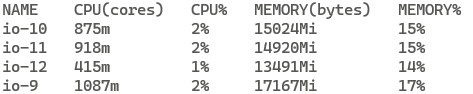
\includegraphics[scale=0.7]{resource-use1.png}
	\caption{میزان مصرف منابع سخت افزاری پلتفرم بدون بار}
	\label{fig: resource use no load}
\end{figure}
\clearpage
\section{حل مسئله و نتایج}
 
پس از پیاده سازی پلتفرم \lr{MLOps} نیاز به ارزیابی آن داریم. هدف از این کار، بررسی قابلیت‌ها و عملکرد این پلتفرم در مدیریت و اجرای مدل‌های یادگیری ماشین به صورت خودکار و پیوسته است. به منظور ارزیابی و تست پلتفرم، سه مسئله مختلف مورد بررسی قرار می‌گیرند. در مسئله اول، از قابلیت \lr{Notebooks} در این پلتفرم استفاده شده است و دو مسئله دیگر به صورت کدهای پایتون نوشته شده‌اند که با بهره‌گیری از \lr{CI/CD}، روی پلتفرم پیاده‌سازی و اجرا می‌شوند. این رویکرد، به ما امکان می‌دهد تا عملکرد پلتفرم را در شرایط مختلف و با استفاده از ابزارهای متفاوت بررسی و ارزیابی کنیم.

\subsection{مسئله تشخیص ارقام}
\subsection{مسئله تحلیل احساسات در بازار سهام}

مسئله اصلی این پروژه تحلیل احساسات در بازار سهام است. هدف این است که با استفاده از نظرات و اخبار اقتصادی، احساسات مثبت و منفی موجود در بازار شناسایی شود و تأثیر آن بر رفتار بازار تحلیل گردد. داده‌های دادگان این مسئله به تجربیات احساس بازار سهام مربوط می‌شود  که از حساب‌های مختلف توئیتر، شامل 5791 توئیت مرتبط با اخبار اقتصادی پیرامون سهام، با دسته‌بندی احساس مثبت و منفی جمع‌آوری شده‌اند. این مجموعه‌داده به دو بخش مثبت و منفی تقسیم می شوند که تعداد موارد منفی 2106 و تعداد موارد مثبت 3685 است. در شکل 
~\ref{fig: stock data}
 ده سطر اول از این داده‌ها به عنوان نمونه نشان داده شده است. راه حل ارائه شده برای حل این مسئله استفاده از شبکه های \lr{LSTM} می باشد. به منظور کنترل و مدیریت این مسلئه از دو خط لوله مجزا برای آموزش و استقرار استفاده شده است. 
\begin{figure}[!b]
	\centering
	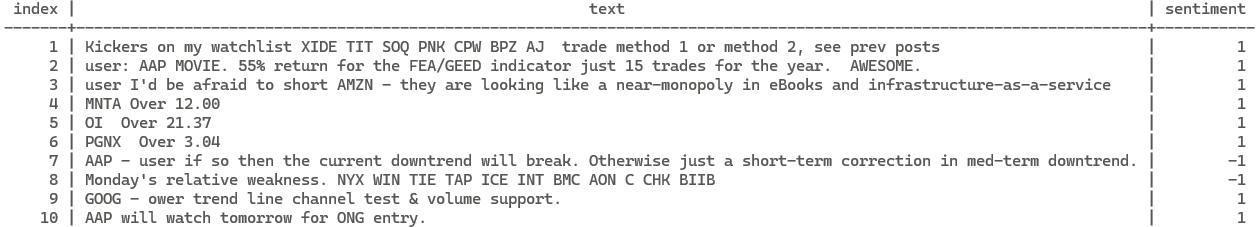
\includegraphics[scale=0.6]{stock-table.png}
	\caption{مجموعه داده احساسات در بازار سهام}
	\label{fig: stock data}
\end{figure}

\subsubsection{خط لوله آموزش}
در این خط لوله از قابلیت کانتینر برای استقرار آسان استفاده شده است و شامل آزمون‌هایی برای اطمینان از عملکرد و دقت راه‌حل‌های پیاده‌سازی شده است که هر کانتینر با ساخت و اجرای فایل و تصویر داکر مربوطه اجرا خواهد شد. هم چنین،‌ برای ساخت خط لوله در بستر پلتفرم لازم است که در ابتدا بخش‌های مختلف پروژه را به مولفه‌های مجزا تقسیم کرد، به طوری که هر مولفه دارای یک فایل داکر بوده و به صورت مجزا به آن نگاه خواهد شد. در این جا ما با سه مولفه سر و کار خواهیم داشت که مراحل پیش‌پردازش، آموزش و آزمایش چرخه‌ی یادگیری ماشین ما خواهند بود. همچنین برای ساخت خط لوله نیاز است تا اسکریپت جداگانه‌ای مربوط با کدهای این بخش که با کتابخانه \lr{kfp} است نوشته شود، تا بتوان با استفاده از تصاویر داکری ساخته شده در هر مولفه، پایپلاین مورد نظر را روی بستر پلتفرم \lr{MLOps} ساخت. در شکل 
~\ref{fig: stock train}
یکی از اجراهای خط لوله \lr{CI/CD} برای مرحله آموزش را مشاهده می کنید.
\begin{figure}[!t]
	\centering
	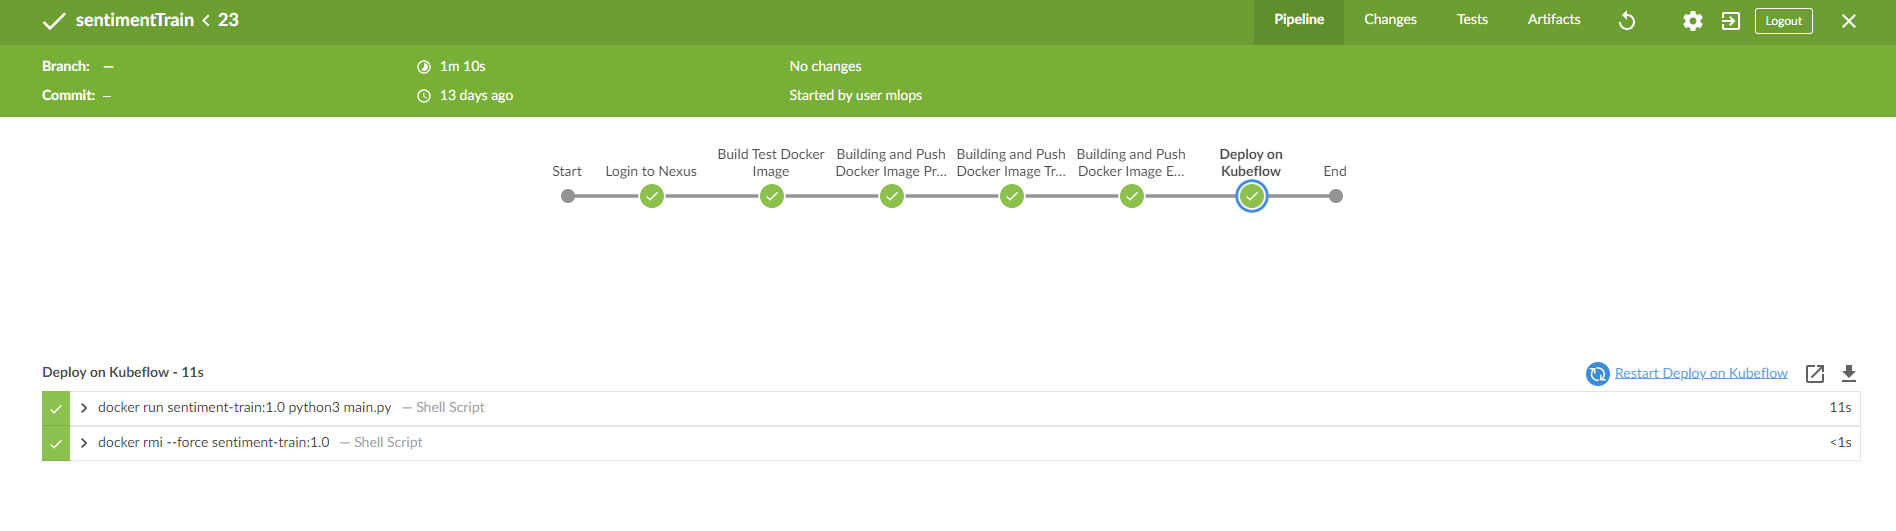
\includegraphics[scale=0.4]{stock-train.png}
	\caption{خط لوله آموزش مسئله تحلیل احساسات در بازار سهام}
	\label{fig: stock train}
\end{figure}

همان طور که می بینید این خط لوله شامل چندین بخش از جمله پیش پردازش،‌ آموزش،‌ ارزیابی و پیاده سازی روی بستر پلتفرم \lr{MLOps} با استفاده از \lr{Kubeflow Pipeline} می باشد.


پیش پردازش شامل چندین مرحله کلیدی است که داده‌ها را برای مدل‌سازی آماده می‌کند. این مراحل شامل تغییر برچسب‌ها به مقادیر دسته‌ای، تمیز کردن متن از کاراکترها و کلمات بی‌معنی، تقسیم داده‌ها به دو بخش آموزش و ارزیابی، و تبدیل متن به دنباله‌هایی از کلمات است.  همچنین، واژگان با استفاده از تعبیه‌گرهای پیش‌آموزش داده شده \lr{GloVe} به بردارهایی تبدیل می‌شوند که حاوی اطلاعات معنایی و ارتباطی کلمات هستند. فایل‌های تعبیه‌گر \lr{GloVe} از \lr{MinIO} دانلود شده و بردارهای تعبیه برای واژگان موجود در داده‌های آموزش ساخته می‌شود. این بردارها سپس برای ایجاد یک ماتریس تعبیه جهت استفاده در شبکه عصبی به کار می‌روند. داده‌های تعبیه‌شده و سایر داده‌های پردازش‌شده نیز در \lr{MinIO} ذخیره می‌شوند تا در مراحل بعدی مورد استفاده قرار گیرند. برای ذخیره و بازیابی داده‌ها، از دو ابزار اصلی \lr{MinIO} و \lr{PostgreSQL} استفاده می‌شود. در کلاس پیش‌پردازش، فایل‌های تعبیه‌گر \lr{GloVe} را از \lr{MinIO} دانلود و بردارهای تعبیه برای واژگان موجود در داده‌های آموزش ساخته می‌شود. همچنین، داده‌های پردازش‌شده نیز در \lr{MinIO} ذخیره می‌شوند. \lr{PostgreSQL} نیز برای بازیابی مجموعه‌داده اولیه به کار می‌رود، به طوری که داده‌ها از پایگاه‌داده خوانده شده و برای پردازش و آماده‌سازی بیشتر به کلاس پیش‌پردازش منتقل می‌شوند. 


در بخش آموزش از شبکه‌های حافظه کوتاه-مدت بلند\footnote{\lr{Long short-term memory (LSTM)}} به دلیل توانایی‌شان در درک و پردازش توالی‌های زمانی طولانی‌مدت، برای تحلیل احساسات متنی استفاده شده است. برخلاف مدل‌های سنتی که ممکن است نتوانند ارتباطات طولانی‌مدت بین کلمات را به خوبی درک کنند، \lr{LSTM} با استفاده از سلول‌های حافظه و مکانیزم‌های دروازه‌ای خود، قادر است اطلاعات مهم را حفظ و اطلاعات غیرضروری را فراموش کند. برای استفاده از \lr{LSTM} در تحلیل احساسات، از داده های پیش پردازش شده که در \lr{MinIO} ذخیره‌سازی شده بود استفاده می شود. پس از آماده‌سازی داده‌ها، مدل \lr{LSTM} با تعریف لایه‌های مختلف از جمله لایه‌های تعبیه‌گر، لایه‌های \lr{LSTM} دوطرفه و لایه‌های چگال ساخته می‌شود. این لایه‌ها به مدل امکان می‌دهند تا وابستگی‌های معنایی و زمانی بین کلمات را بهتر درک کند. علاوه بر این،‌ به منظور جلوگیری از بیش برازش از لایه های \lr{Dropout} با نرخ \lr{0.2} استفاده شده است.

در انتها پس از آموزش، مدل با استفاده از مجموعه دادگان ارزیابی، بررسی می شود. معیارهای ارزیابی مدل نیز دقت آن می باشد. در صورتی که بررسی های انجام شده از دقت مدل های گذشته بیشتر بود، مدل در \lr{MinIO} ذخیره‌سازی می شود.

به منظور اجرا چرخه یادگیری ماشین گفته شده این چرخه با استفاده از کتابخانه \lr{kfp} روی بستر پلتفرم اعمال شده تا فرآیند پیش پردازش،‌ آموزش و ارزیابی مدل را روی پلتفرم انجام دهد (شکل ~\ref{fig: stock workflow}).

\begin{figure}[t]
	\centering
	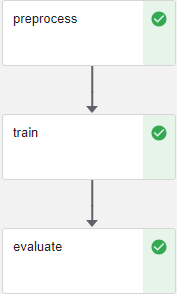
\includegraphics[scale=0.8]{stock-workflow.png}
	\caption{چرخه کاری آموزش مسئله تحلیل احساسات در بازار سهام}
	\label{fig: stock workflow}
\end{figure}

\subsubsection{خط لوله استقرار}
همان طور که در شکل 
~\ref{fig: stock serve}
مشاهده می کنید، اجرای خط لوله استنتاج مدل در پلتفرم با استفاده از \lr{Kserve} شامل چند مرحله کلیدی است. ابتدا، یک فایل پیکربندی برای \lr{Kserve} ایجاد می‌شود که جزئیات مدل، مسیر مدل ذخیره شده و هرگونه مراحل پیش‌پردازش یا پس‌پردازش لازم را مشخص می‌کند. سپس، یک جزء\footnote{\lr{Component}}  \lr{Kserve} با استفاده از کتابخانه \lr{kfp} ایجاد می‌شود که از فایل پیکربندی \lr{YAML} استفاده می‌کند. این جزء باید شامل منطق لازم برای استقرار مدل، مدیریت درخواست‌های ورودی و ارائه پیش‌بینی‌ها باشد. پس از ایجاد جزء، با استفاده از \lr{Kubeflow Piepline} روی بستر پلتفرم پیاده‌سازی می‌شود. این شامل تعریف وابستگی‌ها بین اجزا است تا اطمینان حاصل شود که جزء استقرار مدل پس از اجزا آموزش مدل و ارزیابی اجرا می‌شود. در نهایت، ارتباط با \lr{Endpoint} از طریق \lr{REST API} انجام می‌شود. این فرآیند به تحلیلگران اجازه می‌دهد تا مدل‌های یادگیری ماشین را به طور مؤثر استقرار و مدیریت کنند و از ویژگی‌های پیشرفته مانند مقیاس‌پذیری خودکار، تعادل بار و پایش عملکرد بهره‌مند شوند. 
\begin{figure}[!t]
	\centering
	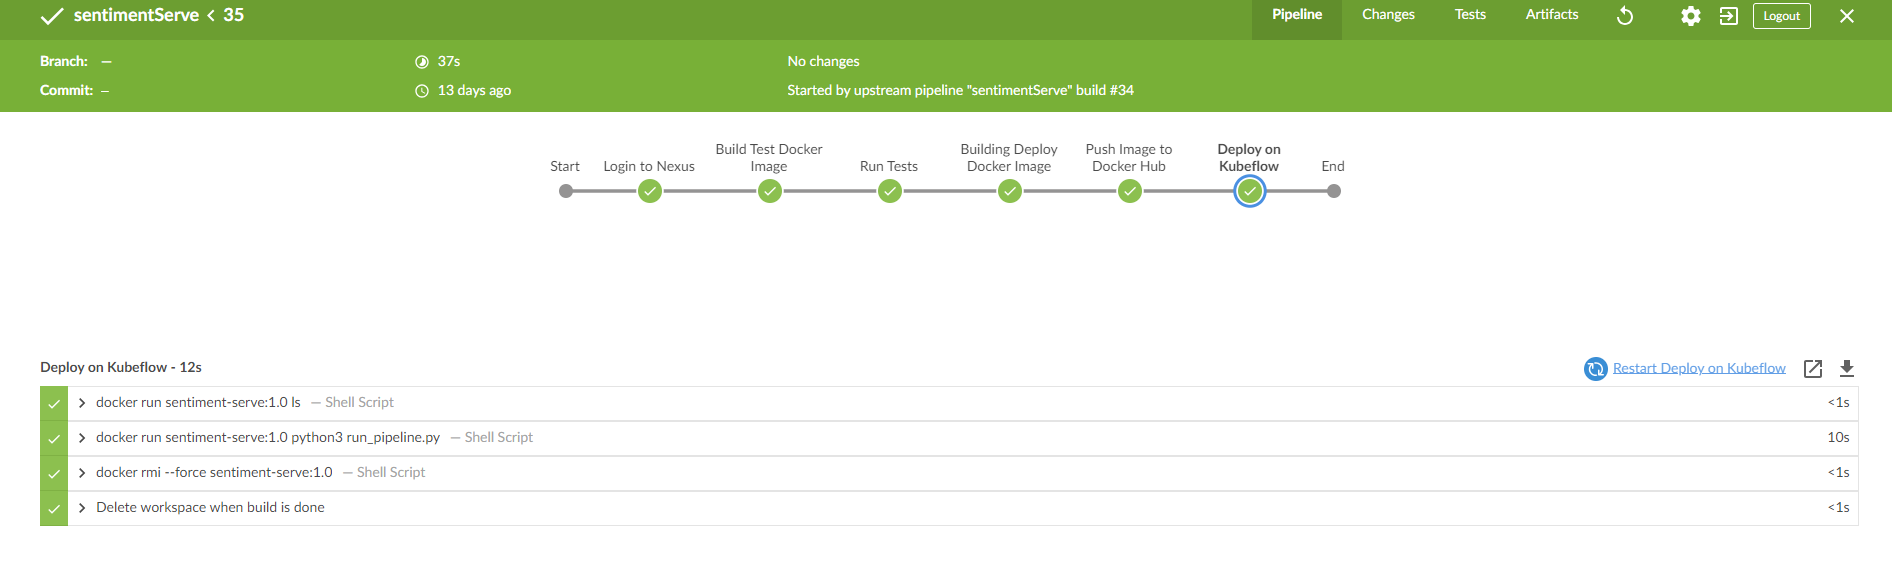
\includegraphics[scale=0.4]{stock-serve.png}
	\caption{خط لوله استقرار مسئله تحلیل احساسات در بازار سهام}
	\label{fig: stock serve}
\end{figure}


\subsubsection{نتایج}
از آنجا که دقت و کارایی مدل هدف پیاده‌سازی مسئله نبوده و صرفا هدف ما تست عملکردی پلتفرم می باشد، ملاک ارزیابی ما زمان اجرا خط لوله ها و چرخه یادگیری ماشین،‌ مدت زمان پاسخ و میزان مصرف منابع می باشد. 
در جدول 
~\ref{tb: stock pipeline time}
زمان اجرای هر بخش را برای اجرای یک تغییر نشان داده شده است. کل مدت زمان آموزش تا استقرار مدل مجموعا 392 ثانیه می باشد.
توجه داشته باشید که این زمان بدون لحاط زمان کش می باشد. در صورتی که تغییر در یک جزء صورت می گیرد تنها آن جزء اجرا شده و بقیه اجزا از حافظه نهان برای اجرا آن استفاده می کنند. 
\begin{table}
	\centering
	\caption{زمان اجرا خط لوله ها \lr{CI/CD} و چرخه یادگیری ماشین در مسئله تحلیل احساسات در بازار سهام }
	\label{tb: stock pipeline time}
	\begin{tabular}{|c|c|}
		\hline
		زمان (ثانیه) & خط‌لوله  \\ \hline
		\lr{70} &  \lr{CI/CD} آموزش  \\ \hline
		\lr{187} &  چرخه کاری آموزش  \\ \hline
		\lr{37} &  \lr{CI/CD} استقرار  \\ \hline
		\lr{98} & چرخه کاری استقرار  \\ \hline
	\end{tabular}
\end{table}

به منظور تست مدل استقرار یافته،‌ به صورت همزمان به آن درخواست داده و زمان پاسخ و میزان مصرف \lr{CPU} را گزارش کرده ایم. نتایج این تست در جدول 
~\ref{tb: stock req}
گزارش شده است. 

\begin{table}
	\centering
	\caption{تست استنتاج مدل مسئله تحلیل احساسات در بازار سهام}
	\label{tb: stock req}
	\begin{tabular}{|c|c|c|}
		\hline
		\lr{CPU (mili cores)} &  زمان پاسخ (ثانیه) & تعداد  \\ \hline
		\lr{24}  & \lr{4.16} & \lr{1} \\ \hline
		\lr{110}  & \lr{4.59} & \lr{4} \\ \hline
		\lr{290}  & \lr{5.51} & \lr{10} \\ \hline
		\lr{387}  & \lr{6.48} & \lr{16} \\ \hline
		\lr{566}  & \lr{8.91} & \lr{32} \\ \hline
		\lr{845} & \lr{13.99} & \lr{64} \\ \hline
		\lr{1142}  & \lr{11.86} & \lr{100} \\ \hline
		\lr{1338}  & \lr{14.09} & \lr{128} \\ \hline
		\lr{1689}  & \lr{14.45} & \lr{256} \\ \hline
		\lr{2090} & \lr{15.8} & \lr{512} \\ \hline
	\end{tabular}
\end{table}

نتایج در تعداد درخواست ها بالا به دلیل استفاده از تکنیک مقیاس پذیری خودکار در پلتفرم با استفاده از ابزارهای \lr{Istio} و \lr{Knative} مناسب است ولی در تعداد درخواست های پایین مناسب نمی باشد. به منظور رفع این مشکل از سرویس \lr{LoadBalancer} در خوشه کوبرنتیز استفاده شده است که نتایج آن را در شکل 
~\ref{fig: stock time request}
مشاهده می کنید. در این روش به دلیل استفاده نکردن از تکنیک مقیاس پذیری خودکار،‌ زمان درخواست ها در سناریوهایی که تعداد درخواست های همزمان زیاد می باشد، مناسب نمی باشد.

\begin{figure}[t]
	\centering
	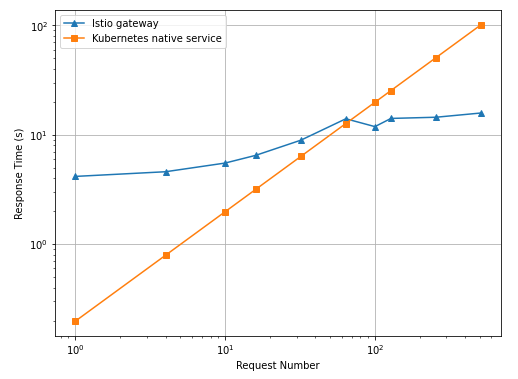
\includegraphics[scale=0.8]{stock-time-req.png}
	\caption{زمان استنتاج مدل در مسئله تحلیل احساسات دربازار سهام}
	\label{fig: stock time request}
\end{figure}








\subsection{مسئله توصیه گر کتاب}